% !TEX encoding = UTF-8
% !TEX program = pdflatex
% !TEX root = InformationRetrieval.tex
% !TEX spellcheck = it-IT

%section Valutazione di un sistema su più topic

\section{Misure con più gradi di rilevanza}

Volendo si può definire una scala di rilevanza per i vari documenti, come \textit{abbastanza rilevante} o \textit{parzialmente rilevante}, ma le misure finora viste non ne tengono conto.

Ad ogni grado di rilevanza è possibile associare un peso, che prende il nome di \textbf{relevance weight}. Un esempio di \textbf{multigraded relevance}:

\begin{itemize}
	\item \textit{Highly Relevenant} $\to 15$
	\item \textit{Fairly Relevenant} $\to 10$
	\item \textit{Partially Relevenant} $\to 5$
	\item \textit{Not Relevenant} $\to 0$
\end{itemize}

\noindent Il sistema di pesi prende il nome di relevance schema e può variare.

\subsection{Cumulative Gain (CG)}

\`E una delle famiglie di misure più utilizzate nell'Information Retrieval, si basa su giudizi di rilevanza multigrado e sfrutta i pesi assegnati ai giudizi di rilevanza per calcolare l'efficacia di un sistema (o di una run).

Utilizzando più gradi di rilevanza, l'assesment di una run diventa leggermente diversa:

\begin{figure}[htbp]
	\centering
	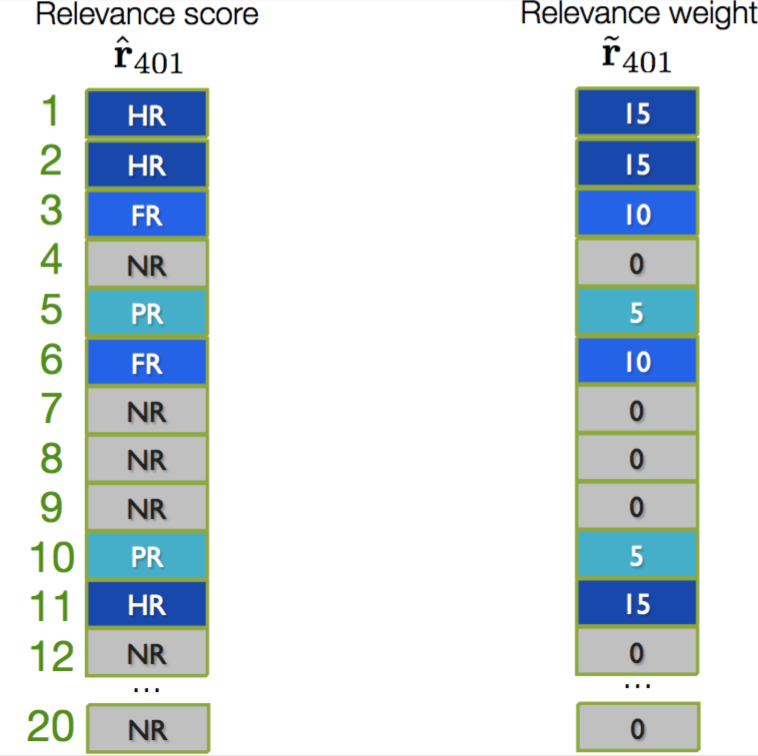
\includegraphics[width=0.5\textwidth]{images/l16-fig-1.png}
\end{figure}

\noindent Formalmente, sia $R(t)$ una run di lunghezza $N \in \mathbb{N}^+$, dove $t$ è un dato topic, $RB_t$ la sua recall base e $j \in \mathbb{N}^+ | 1 \leq j \leq N$. $CG[j]$ è definito come:

$$
CG[j] = cg_{r_t}[j] = \sum\limits_{k=1}^j \tilde{r}_t[k]
$$

\noindent Ad esempio si ha che, per la run dell'immagine precedente viene calcolato con:

$$
CG[j] = cg_{r_t}[j] = \sum\limits_{k=1}^{20} \tilde{r}_{401}[k] = 75
$$

\noindent ovvero è la somma dei pesi dei vari giudizi.

Al variare di del rango $k$ è possibile fare il plot del cumulative gain per farsi un'idea di massima dell'andamento della run.

\begin{figure}
	\centering
	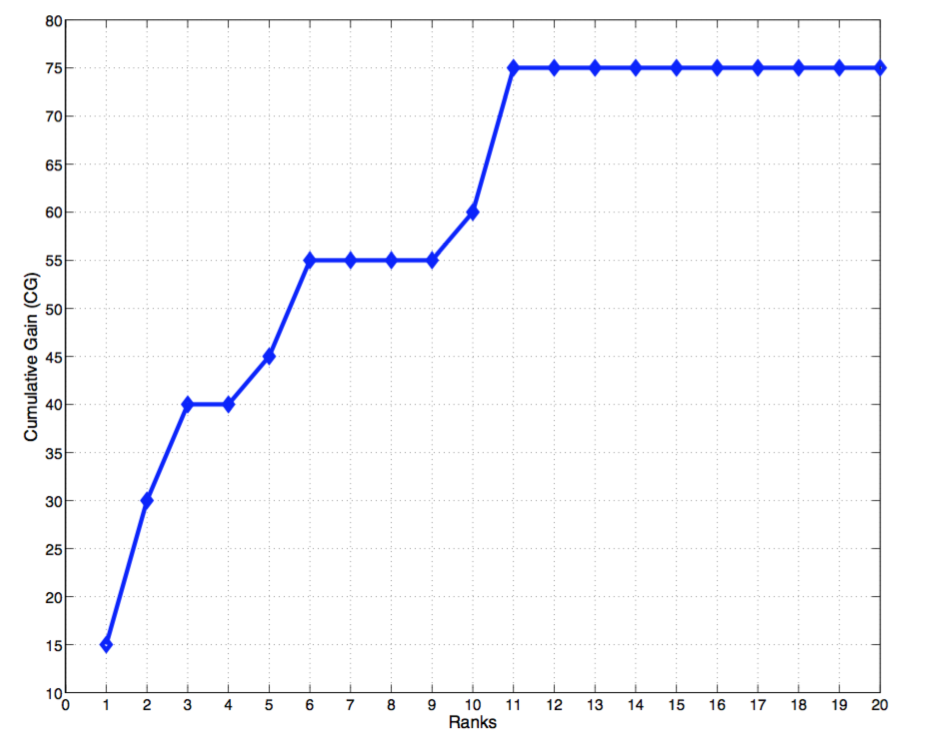
\includegraphics[width=0.4\textwidth]{images/l16-fig-2.png}
\end{figure}

Questa misura, presa così com'è non è top-heavy, ovvero non da maggior peso ai documenti rilevanti che hanno rango diverso. Tuttavia facendo il plot è possibile confrontare due run, evidenziato anche la top-heaviness.

\begin{figure}
	\centering
	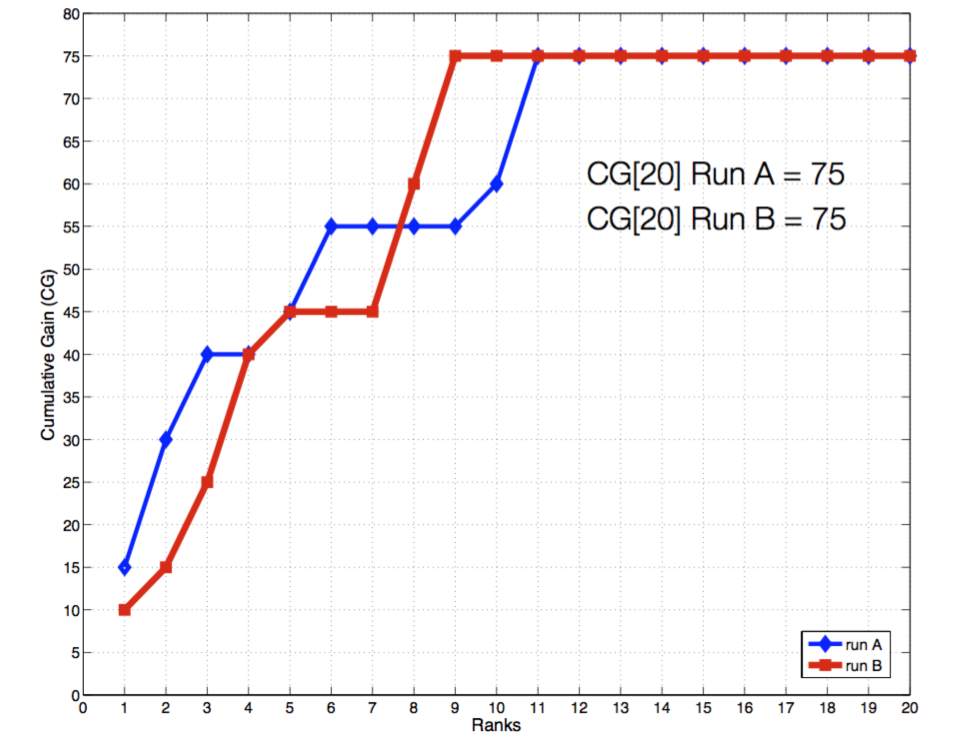
\includegraphics[width=0.4\textwidth]{images/l16-fig-3.png}
	\caption{Da notare che il CG delle run è uguale, ma dalla curva si riesce a capire che la run A a rango 3 recupera documenti più rilevanti della run B.}
\end{figure}

Quindi, per ottenere una misura top-heavy è possibile calcolare il $CG$ con un livello di cut-off.

\subsection{Disconted Cumulative Gain (DCG)}

Questa misura è una variante top-heavy di $CG$ che utilizza una \textbf{discounting function} che riduce progressivamente il peso dei documenti, mano a mano che si avanza nel ranking.

Partendo sempre da una run $R(t)$ di lunghezza $N$ e da una base logaritmica $b \in \mathbb{N}^+$, per tutti i $k \in [1,N]$ il \textbf{discounted gain} è definito come:

$$
dg_{r_t}^b[h] = \begin{cases}
\tilde{r}_t[k] \quad &\text{se } k < b \\
\cfrac{\tilde{r}_t[k]}{\log_b k} &\text{altrimenti}
\end{cases}
$$

\begin{figure}[htbp]
	\centering
	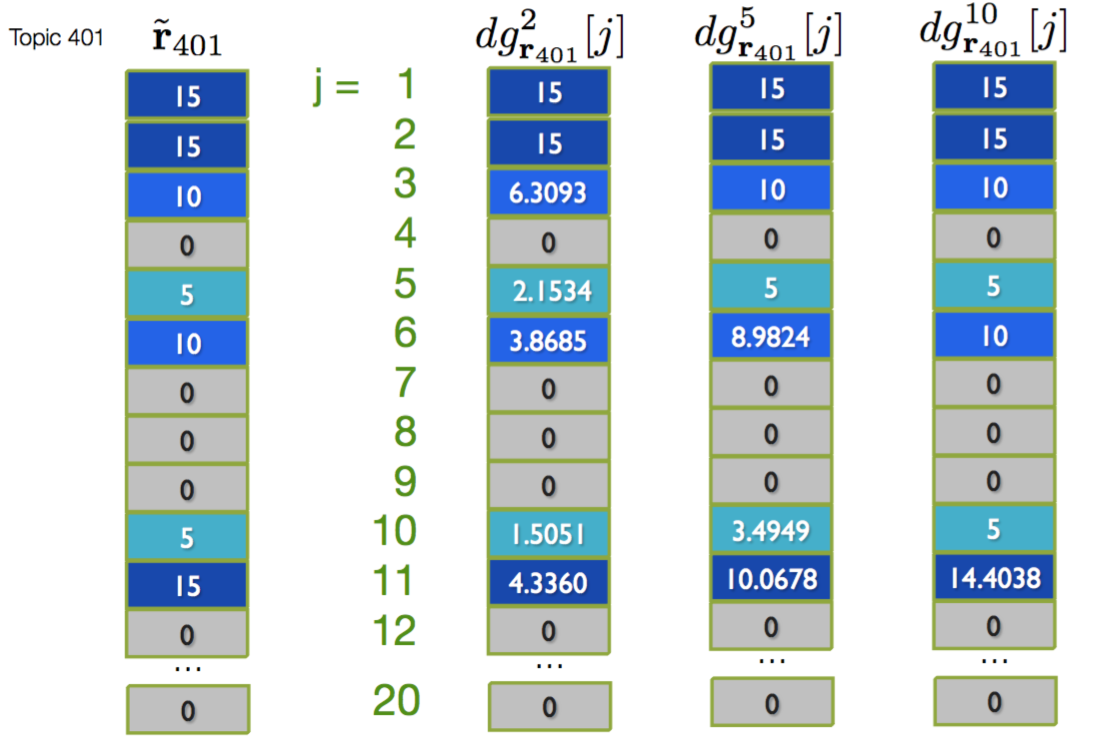
\includegraphics[width=0.4\textwidth]{images/l16-fig-4.png}
	\caption{Esempio di calcolo di discounted gain.}
\end{figure}

La funzione di sconto è utili per modificare la misura sulla base del task da valutare, tipicamente se il task è una ricerca web si utilizza $b=10$, mentre se è una ricerca mobile $b=2$.
Ma $b$ può anche essere utilizzato per discriminare il fatto \textit{utenti pazienti-impazienti}, perché un utente paziente tipicamente guarda più elementi tra i risultati della ricerca.

Una volta calcolato il disconted-gain, il \textbf{Disconted Cumulative Gain} è dato da:

$$
DCG[j] = \sum\limits_{k=1}^{j}dg_{r_t}^b[k]
$$


\begin{figure}[htbp]
	\centering
	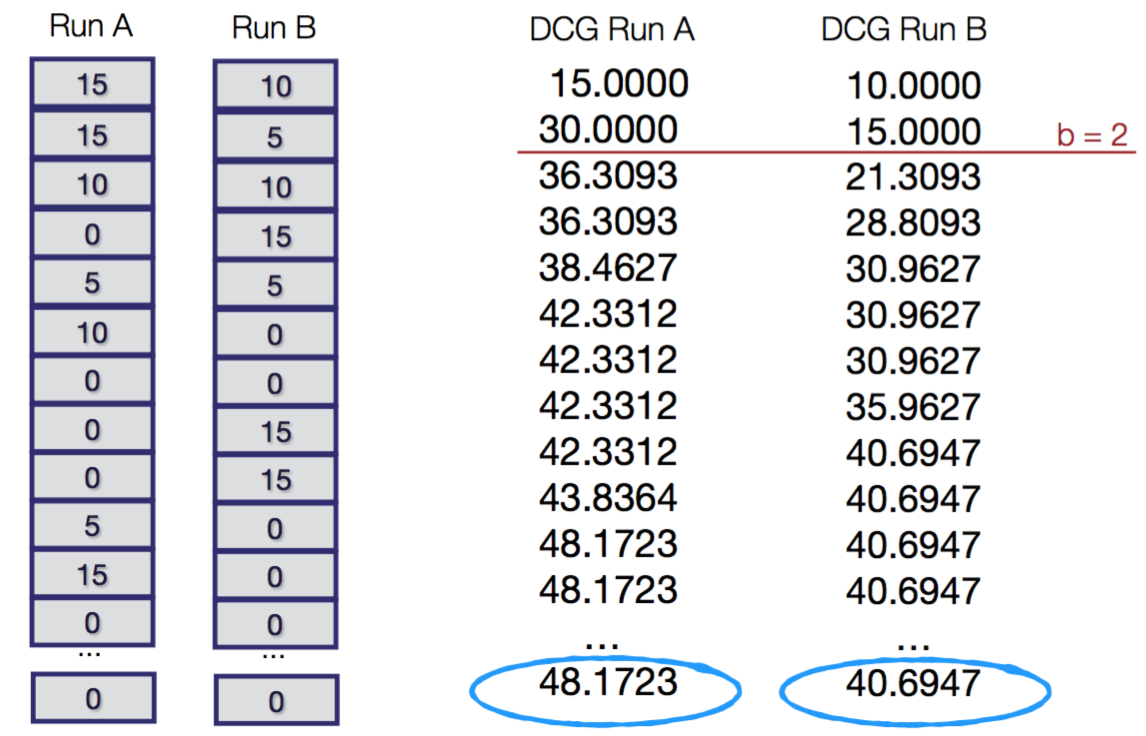
\includegraphics[width=0.6\textwidth]{images/l16-fig-5.png}
	\caption{Esempio di calcolo di DCG.}
\end{figure}

\begin{figure}[htbp]
	\centering
	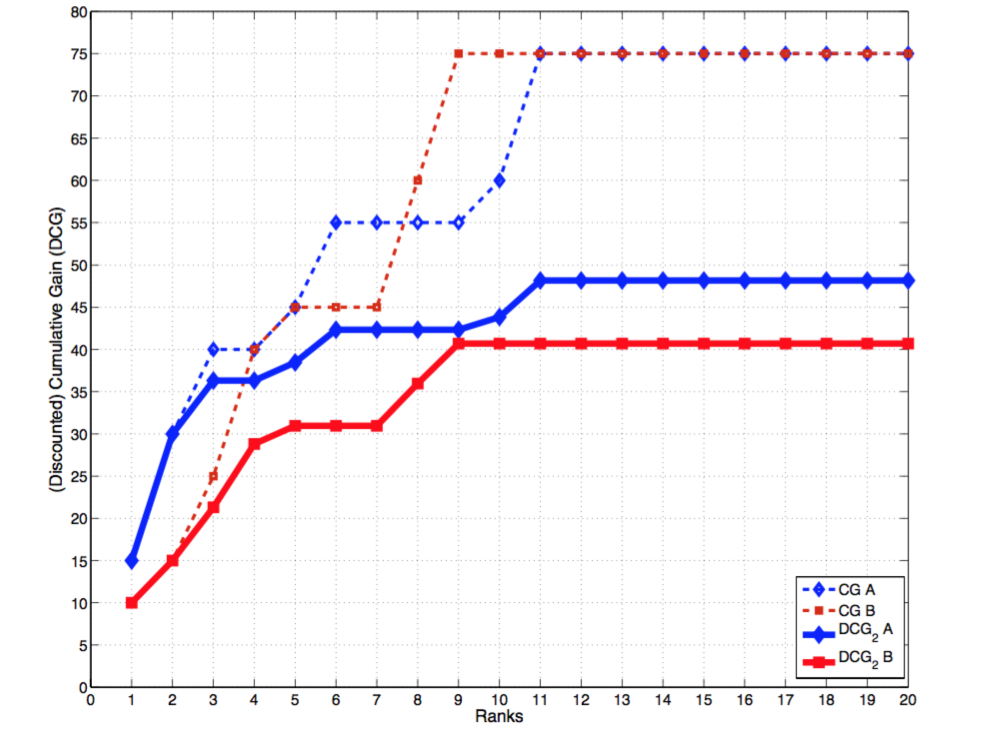
\includegraphics[width=0.4\textwidth]{images/l16-fig-6.png}
	\caption{Plot dei confronti tra le curve.}
\end{figure}

\noindent DCG è quindi una misura top-heavy che può essere calcolato con vari livelli di cut-off che può anche essere adattata ai vari task di ricerca.

C'è però un problema, perché la misura non è compresa tra 0 e 1 e il valore assoluto della misura non dice nulla di particolare, in quanto il massimo varia da topic a topic. \textbf{Attenzione che non ha senso fare la media del DCG per i vari topic}

\subsection{Normalizzazione dei cumulative gain}

\`E una tecnica che permette di portare sia $CG$ che $DCG$ nell'intervallo $[0,1]$, sfruttando il concetto di \textbf{run ideale}, ovvero la miglior run possibile dato un pool e un topic, cioè quella recupera tutti i documenti rilevanti presenti e li ordine per grado di rilevanza.
Quindi calcolando $CG$ o $DCG$ sulla run ideale ottengo il valore massimo, che posso utilizzarlo per normalizzare le misure sulle altre run.

Più formalmente la run ideale $I(t) = i_t$ è una run che soddisfa i seguenti vincoli:

\begin{enumerate}
	\item \textit{recall base}: $\forall t \in T \big | \{ j \in [1,N] | GT(t,i_t[j]) \geq min(REL) \} \big | = RB_t$
	\item \textit{ordinamento}: $\forall t \in T, \forall j,k \in [1,N] | j < k \Rightarrow \hat{i_t}[j] \geq \hat{i_t}[k]$
\end{enumerate}

\begin{figure}[htbp]
	\centering
	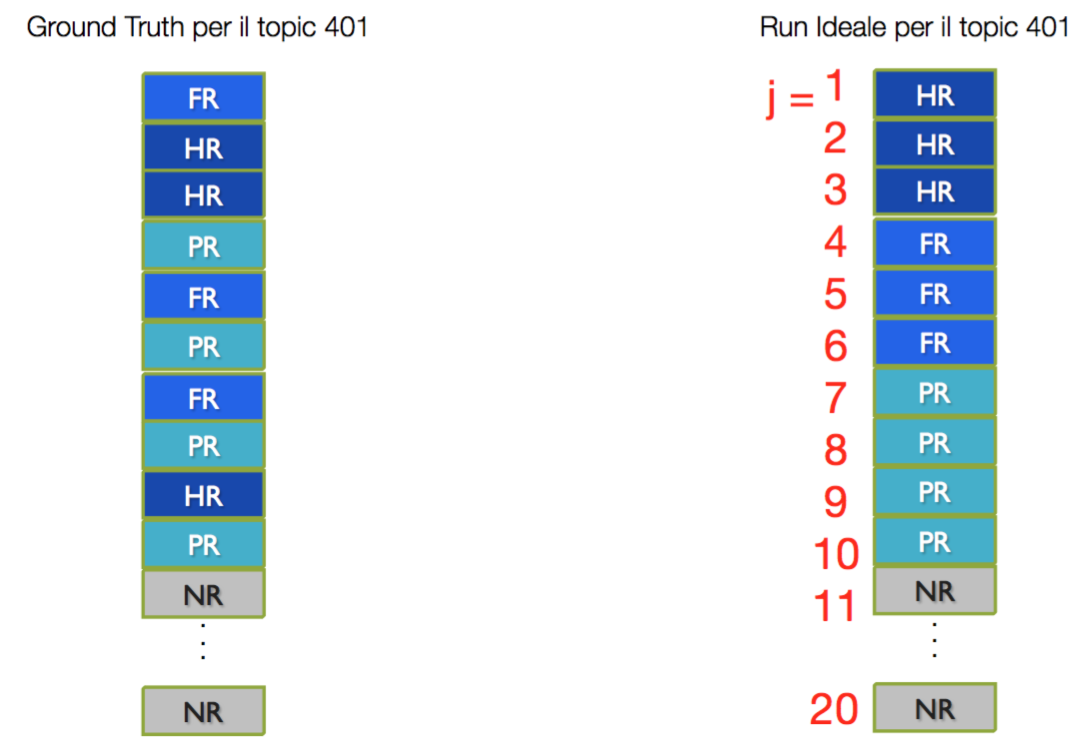
\includegraphics[width=0.4\textwidth]{images/l16-fig-7.png}
	\caption{Esempio di run ideale, da notare che servono solo le informazioni sul ground truth}
\end{figure}

Il \textbf{Cumulative Gain normalizzato (nGC)} viene calcolato con:

$$
nGC[j] = \frac{cg_{r_t}[j]}{cg_{i_t}[j]}
$$

ed in modo simile \textbf{DCG normalizzato} viene calcolato con:

$$
nDCG^b[j] = \frac{\sum_{k=1}^j dg_{r_t}^b[k]}{dg_{i_t}^b[k]}
$$

Riassumendo, $n(D)CG$ è un valore compreso tra 0 e 1 che permette di confrontare diverse run sullo stesso topic e di fare la media dei valori per run cross-topic, in questo caso prende il nome di \textbf{average $n(D)CG$}

Si può inoltre fare l'analisi qualitativa della versione normalizzata, ottenendo così una curva che può anche decrescere, perché dipende sempre dalla run ideale. Si ha quindi che questa curva è più informativa di quelle per le misure non normalizzate, perché quando c'è un punto in cui la curva non normalizzata è costante, non si sa se la mancanza di documenti rilevanti è dovuta al fatto che non ce ne sono più o perché il sistema non riesce a trovarli.
Nel grafico della curva può anche essere plottata la run ottimale, ovvero la run che ha gli stessi documenti della run trovata, ma correttamente ordinati per rilevanza. 
Il confronto grafico con la run ottima/ideale prende il nome di \textbf{failure analysis} del sistema, ovvero di andare a analizzare i punti in cui il sistema che sotto analisi sbaglia maggiormente.

% ci sono dei bellissimi grafici che il tipo non ha messo sulle slide

